% Generated by scripts/build.py from content.yaml. Do not edit by hand.
% !TEX program = lualatex
\documentclass[a4paper,10pt]{article}
\usepackage[margin=1.4cm]{geometry}
\usepackage{enumitem,titlesec,xcolor,fontspec,graphicx,fontawesome5,xurl,needspace}
\urlstyle{same}
\usepackage[hidelinks]{hyperref}
\setlength{\parindent}{0pt}\setlength{\parskip}{4pt}
\setlist[itemize]{noitemsep, topsep=0pt, leftmargin=1.5em}
\setlist[enumerate]{topsep=2pt, itemsep=3pt, leftmargin=1.6em}
\renewcommand{\baselinestretch}{1.05}
\definecolor{primary}{HTML}{27438D}\definecolor{muted}{HTML}{5A5A5A}\definecolor{headerbg}{HTML}{C3DFF1}
\setmainfont{Ubuntu}[Path=fonts/, Extension=.ttf, UprightFont=Ubuntu-L, BoldFont=Ubuntu-B, ItalicFont=Ubuntu-LI, BoldItalicFont=Ubuntu-BI]
\hypersetup{colorlinks=true, urlcolor=primary, linkcolor=primary,
  pdftitle={Vipin Singh, CV}, pdfauthor={Vipin Singh}, pdfsubject={Curriculum Vitae},
  pdfkeywords={Holistic model evaluation, Robustness, Time series forecasting, Spatiotemporal modeling, Multimodal deep learning, Uncertainty quantification, Expert-AI collaboration}}
\titleformat{\section}{\needspace{6\baselineskip}\Large\bfseries\color{primary}}{}{0em}{}[\color{primary}\titlerule]
\titlespacing*{\section}{0pt}{10pt}{3pt}
\newcommand{\entry}[4]{\textbf{#1} \hfill \textcolor{muted}{#3}\\\textcolor{muted}{#2\ifx&#4&\else\ \textbf{\textperiodcentered}\ #4\fi}\par}
\begin{document}
\setlength{\fboxsep}{8pt}
\noindent\colorbox{headerbg}{\parbox{\dimexpr\linewidth-2\fboxsep\relax}{%
  \begin{minipage}[c]{0.2\linewidth}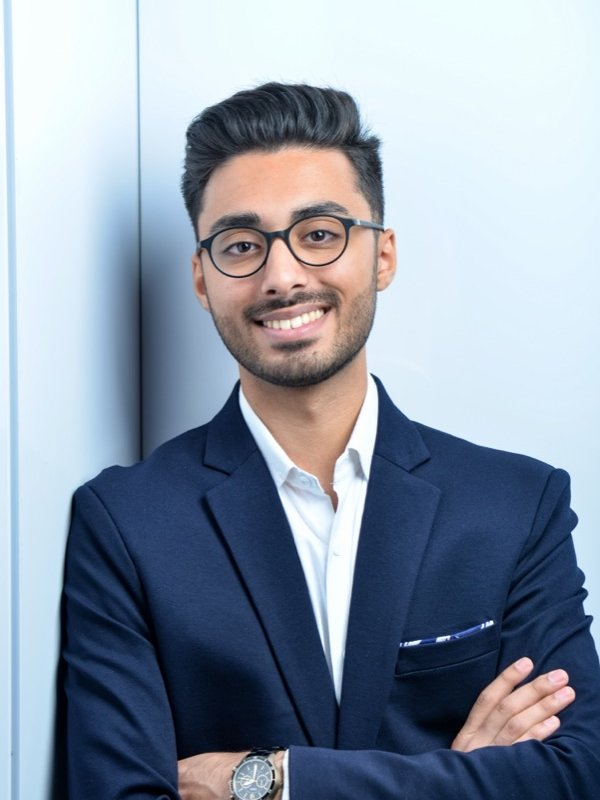
\includegraphics[width=\linewidth]{portrait.jpg}\end{minipage}\hfill
  \begin{minipage}[c]{0.76\linewidth}
    {\LARGE\textbf{Vipin Singh}}\\[3pt]
    \textbf{Data Science Researcher \& Machine Learning Engineer}\\[1pt]
    PhD Candidate in Data Science, Berliner Hochschule für Technik (BHT)\\[5pt]
    \faMapMarker*\ Berlin, Germany\qquad \faEnvelope\ \href{mailto:vipin.singh@bht-berlin.de}{vipin.singh@bht-berlin.de}\\
    \faGlobe\ \href{https://vipin-singh.bio/}{vipin-singh.bio}\qquad \faGithub\ \href{https://github.com/vipin2310}{github.com/vipin2310}\\
    \faLinkedin\ \href{https://www.linkedin.com/in/vipin-singh-131402271}{linkedin.com/in/vipin-singh-131402271}\\
    \faGraduationCap\ \href{https://scholar.google.com/citations?user=9RYzrb4AAAAJ}{Google Scholar}\qquad \faOrcid\ \href{https://orcid.org/0000-0002-4472-8285}{orcid.org/0000-0002-4472-8285}
  \end{minipage}}}

\section*{Profile}
Data science researcher with a background in mathematics and four years of industrial software development. I develop and evaluate machine learning models for environmental applications, from time series forecasting in urban sewer systems to multimodal soil horizon classification and spatiotemporal groundwater level prediction, with a focus on holistic evaluation protocols that assess predictive performance, model complexity and robustness together. Experienced in coordinating work packages in joint research projects with public agencies and industry.

\section*{Experience}
\entry{Research Associate (PhD Candidate), Data Science}{Berliner Hochschule für Technik (BHT)}{Feb 2025 – present}{Berlin, Germany}
\begin{itemize}
  \item Multimodal deep learning models for automatic soil horizon description from profile images and metadata, with BGR.
  \item Spatiotemporal groundwater level prediction at unmonitored locations, with BGR.
  \item Continuation of the RIWWER work packages on time series modeling for urban wastewater management.
  \item Teaching support in data science courses, including preparing material and substitute lecturing.
\end{itemize}
\entry{Student Research Assistant, Data Science}{Berliner Hochschule für Technik (BHT)}{Dec 2023 – Jan 2025}{Berlin, Germany}
\begin{itemize}
  \item Machine learning models for time series forecasting in urban wastewater management.
  \item Evaluation protocols for predictive performance, model complexity and robustness to data perturbations.
  \item Coordination of the AI work package in the RIWWER research project.
\end{itemize}
\entry{Software Developer, Industrial Image Processing}{NeuroCheck GmbH}{Oct 2018 – Aug 2022}{Stuttgart, Germany}
\begin{itemize}
  \item Image processing and computer vision algorithms for industrial quality inspection systems (C\#, .NET).
  \item Custom image processing modules and plugins for the NeuroCheck software.
  \item Tailored solutions for clients together with engineers and quality assurance specialists.
\end{itemize}
\entry{Intern, System Integration}{Thinking Objects GmbH}{May 2016}{Stuttgart, Germany}


\section*{Education}
\entry{PhD in Data Science (ongoing)}{Berliner Hochschule für Technik (BHT)}{Feb 2025 – present}{}
\begin{itemize}
  \item Supervisor: Prof. Dr. Felix Bießmann
\end{itemize}
\entry{M.Sc. Data Science}{Berliner Hochschule für Technik (BHT)}{Oct 2022 – Jan 2025}{}
\begin{itemize}
  \item Thesis: \textit{Time Series Modeling for Urban Water Management}
  \item Final grade: 1.0 (German scale, 1.0 is best)
\end{itemize}
\entry{B.Sc. Mathematics}{Hochschule für Technik Stuttgart}{Sep 2018 – Aug 2022}{}
\begin{itemize}
  \item Thesis: \textit{Development of a Deflectometry-based Inspection System for Reflective Surfaces}
  \item Final grade: 1.3 (German scale, 1.0 is best)
\end{itemize}

\section*{Research Projects}
\textbf{Groundwater level prediction at unmonitored locations} \textcolor{muted}{(2025–present, with BGR)}\\
Can a dense monitoring network predict groundwater levels at future times and at locations without a well, and what limits it? With BGR, we benchmark temporal, spatial and coupled models for Brandenburg under one evaluation protocol. Manuscript in preparation.\par\smallskip
\textbf{SoilNet, AI-assisted soil horizon description} \textcolor{muted}{(2025–present, with BGR)}\\
Describing soil horizons from profile images is slow and varies between experts. SoilNet mirrors the experts' annotation workflow, and in a user study, experts working with the SoilNet App annotated more accurately and more consistently. \href{https://soilnet.demo.calgo-lab.de/}{Live demo} \textbf{\textperiodcentered} \href{https://github.com/calgo-lab/BGR}{Code} \textbf{\textperiodcentered} \href{https://www.bgr.bund.de/}{BGR}\par\smallskip
\textbf{RIWWER, resilient forecasting for urban sewer systems} \textcolor{muted}{(2023–present, with University of Duisburg-Essen and partners)}\\
Combined sewer systems overflow during heavy rain. In the joint project RIWWER, I coordinated the AI work package: forecasting models for rain basins that stay robust to sensor failures and run both in the cloud and on embedded FPGAs at the edge. \href{https://riwwer.demo.calgo-lab.de/}{Live demo} \textbf{\textperiodcentered} \href{https://github.com/calgo-lab/resilient-timeseries-evaluation}{Code} \textbf{\textperiodcentered} \href{https://www.riwwer.fraunhofer.de/}{Project}\par\smallskip

\section*{Publications}
\begin{enumerate}
  \item \textbf{Vipin Singh}, Joey Prüssing, Teodor Chiaburu, Einar Eberhardt, Sina Hesse, Stefan Broda, Frank Haußer, Felix Bießmann. \textit{SoilNet App: AI-Assisted Expert-level Annotations of Soil Horizons}. Proceedings of the 35th International Joint Conference on Artificial Intelligence (IJCAI-ECAI 2026), Demo Track, 2026. \href{https://doi.org/10.24963/ijcai.2026/993}{\nolinkurl{doi:10.24963/ijcai.2026/993}}
    \begin{itemize}
      \item \textit{Summary:} A web-based demonstrator that guides experts through the tasks needed for expert-level soil horizon annotations from profile images. A user study with annotation experts shows that collaborating with the model increases expert performance and inter-annotator consistency.
      \item \textit{My contribution:} Conceptualization, Methodology, Software, Formal analysis, Investigation, Writing – Original Draft, Visualization
    \end{itemize}
  \item \textbf{Vipin Singh}, Tianheng Ling, Peter Ghaly, Felix Grimmeisen, Gregor Schiele, Felix Bießmann. \textit{A Resilient Solution for Sewer Overflow Monitoring Across Cloud and Edge}. Proceedings of the 35th International Joint Conference on Artificial Intelligence (IJCAI-ECAI 2026), Demo Track, 2026. \href{https://doi.org/10.24963/ijcai.2026/994}{\nolinkurl{doi:10.24963/ijcai.2026/994}}
    \begin{itemize}
      \item \textit{Summary:} A web-based demonstrator that integrates our deep learning forecasting methods for combined sewer overflow monitoring across cloud and edge. Its interactive dashboard stays usable during network outages, enabling timely preventive action during extreme rainfall.
      \item \textit{My contribution:} Conceptualization, Methodology, Software, Formal analysis, Investigation, Writing – Original Draft, Visualization, Project administration
    \end{itemize}
  \item \textbf{Vipin Singh}$^*$, Teodor Chiaburu$^*$, Einar Eberhardt, Stefan Broda, Joey Prüssing, Frank Haußer$^\dagger$, Felix Bießmann$^\dagger$. \textit{SoilNet: A multimodal multitask model for hierarchical classification of soil horizons}. Geoderma 466, 117684, 2026. \href{https://doi.org/10.1016/j.geoderma.2026.117684}{\nolinkurl{doi:10.1016/j.geoderma.2026.117684}} {\small\textcolor{muted}{($^*$equal contribution; $^\dagger$equal supervision)}}
    \begin{itemize}
      \item \textit{Summary:} A multimodal multitask neural network for automatic soil horizon classification from profile images and metadata. Its grey-box design mirrors the annotation procedure used by domain experts.
      \item \textit{My contribution:} Conceptualization, Methodology, Software, Formal analysis, Investigation, Writing – Original Draft, Visualization
    \end{itemize}
  \item Teodor Chiaburu, \textbf{Vipin Singh}, Frank Haußer$^\dagger$, Felix Bießmann$^\dagger$. \textit{Uncertainty-Guided Expert-AI Collaboration for Efficient Soil Horizon Annotation}. CLEAR-AI Workshop at the European Conference on Artificial Intelligence (ECAI 2025), 2025. \href{https://arxiv.org/abs/2509.24873}{\nolinkurl{arXiv:2509.24873}} {\small\textcolor{muted}{($^\dagger$equal supervision)}}
    \begin{itemize}
      \item \textit{Summary:} Applies conformal prediction to SoilNet to obtain calibrated uncertainty estimates, and shows the benefit of calibration in a simulated human-in-the-loop annotation pipeline with a limited query budget.
      \item \textit{My contribution:} Validation
    \end{itemize}
  \item Tianheng Ling$^*$, \textbf{Vipin Singh}$^*$, Chao Qian, Felix Bießmann, Gregor Schiele. \textit{Automated Energy-Aware Time-Series Model Deployment on Embedded FPGAs for Resilient Combined Sewer Overflow Management}. 2025 IEEE International Smart Cities Conference (ISC2), 2025. \href{https://doi.org/10.1109/ISC266238.2025.11293267}{\nolinkurl{doi:10.1109/ISC266238.2025.11293267}} {\small\textcolor{muted}{($^*$equal contribution)}}
    \begin{itemize}
      \item \textit{Summary:} Deploys time series models on resource-constrained edge devices for combined sewer monitoring, with an automated hardware-aware pipeline that optimizes model configurations for energy consumption and predictive performance.
      \item \textit{My contribution:} Methodology, Software, Validation, Writing – Review \& Editing, Visualization
    \end{itemize}
  \item \textbf{Vipin Singh}, Tianheng Ling, Teodor Chiaburu, Felix Bießmann. \textit{Evaluating Time Series Models for Urban Wastewater Management: Predictive Performance, Model Complexity and Resilience}. 2025 10th International Conference on Smart and Sustainable Technologies (SpliTech), 2025. \href{https://doi.org/10.23919/SpliTech65624.2025.11091801}{\nolinkurl{doi:10.23919/SpliTech65624.2025.11091801}}
    \begin{itemize}
      \item \textit{Summary:} A protocol for evaluating neural forecasting architectures for combined sewer systems on predictive performance, model complexity and robustness to data perturbations, including peak events and a comparison of global and local modeling paradigms.
      \item \textit{My contribution:} Conceptualization, Methodology, Software, Formal analysis, Investigation, Writing – Original Draft, Visualization, Project administration
    \end{itemize}
  \item \textbf{Vipin Singh}, Tianheng Ling, Teodor Chiaburu, Felix Bießmann. \textit{Data-driven Modeling of Combined Sewer Systems for Urban Sustainability: An Empirical Evaluation}. 2nd Workshop on Public Interest AI at the 47th German Conference on AI (KI 2024), CEUR Workshop Proceedings 3958, 2024. \href{https://arxiv.org/abs/2408.11619}{\nolinkurl{arXiv:2408.11619}}
    \begin{itemize}
      \item \textit{Summary:} Compares neural time series models for forecasting rain basin filling levels during network outages, contrasting global models with access to all sensors against local models restricted to nearby sensors.
      \item \textit{My contribution:} Conceptualization, Methodology, Software, Formal analysis, Investigation, Writing – Original Draft, Visualization, Project administration
    \end{itemize}
\end{enumerate}
\section*{Service}
Member of the student council (Fachschaftsrat), Department VI, Berliner Hochschule für Technik (BHT) \textcolor{muted}{(during M.Sc. studies)}. Events, help desks and onboarding for students; logistics of the student learning room.

\section*{Skills}
\textbf{Programming:} Python, C\#, Java\\
\textbf{Machine learning:} PyTorch, scikit-learn, OpenCV, pandas, NumPy\\
\textbf{Tools:} Git, Linux, Docker, Kubernetes
\section*{Languages}
\textbf{German:} Native \quad\textbf{\textperiodcentered}\quad \textbf{English:} Fluent \quad\textbf{\textperiodcentered}\quad \textbf{Hindi:} Proficient

\vfill{\footnotesize\textcolor{muted}{Last updated 2026-10-09. Current version: \href{https://vipin-singh.bio/}{vipin-singh.bio}}}
\end{document}
